\section{Theory}

\subsection{Introduction}
When $\alpha$ particles strike a thin gold foil, some of the particles experience Coulombic repulsion from the Au nuclei and get scattered from the original direction depending on their impact parameter (the perpendicular distance from the axis of the nucleus) (Fig. \ref{1}). However, the number of particles which experience significantly large scattering angles ($\theta$) or even get scattered back ($\theta=180^\circ$) are quite small $\sim 1/2000$. This was explained by Rutherford as the entire positive charge of the atom being concentrated in a very tiny region at the center, which led to the discovery of the nucleus.

\begin{figure}
    \centering
    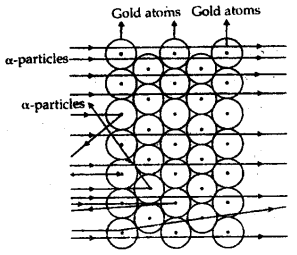
\includegraphics[width=0.9\columnwidth]{images/scat.PNG}
    \caption{Scattering of $\alpha$-particles on a block of Gold atoms visualised}
    \label{1}
\end{figure}

\subsection{Scattering Rate and Cross Section}

The angular distribution of scattering cross section is given by $\frac{d\sigma}{d\Omega}$, which is the amount of scattering per soild angle. Let us denote $N(\theta)$ as the number of particles scattered per unit time per unit solid angle.

Rutherford's scattering formula (in a non-relativistic scenario) can be derived as,

\begin{align}
    \frac{d\sigma}{d\Omega} = \left(\frac{Z_1 Z_2e^2}{4\pi\epsilon_0} \frac{1}{4E}\right)^2 \frac{1}{\sin^4(\frac{\theta}{2})}
\end{align}

where $Z_1$ and $Z_2$ are the atomic numbers of the two interacting particles, $E$ is the kinetic energy of the incoming particle and $\theta$ is the scattering angle. If $\alpha$ particles ($Z=2$) are emitted at a rate $N_0$ with energy $E$ on a material with atomic number $Z$, the scattering rate is given by

\begin{align} \label{eq:2}
    N(\theta) = \frac{N_0Ze^4}{(8\pi\epsilon_0)^2 E^2} \frac{c_F d_F}{\sin^4(\frac{\theta}{2})}
\end{align}

where $c_F$ is the atomic concentration in the foil and $d_F$
the thickness of the foil.

Due to the dependence of the scattering rate on the inverse 4th power of $sin(\theta/2)$, the value of $N(\theta)$ rapidly declines after the singularity at $\theta=0$. 
Higher scattering angles result in very tiny counting
rates, hence in order to achieve an acceptable level of
precision, the gate times $t(\theta)$ for calculating the counting rate $N (\theta)$ must be raised with rising angle $\theta$. As a result, in the initial portion of the experiment, we begin at 5$^\circ$ and gradually increase the gate duration as we climb higher until 30$^\circ$.

\subsubsection*{Space correction for Scattering Rate}
The scattering rates $N_d(\theta)$ are determined by recording the pulse counts $n(\theta)$ for a given angle $\theta$ over a gate time $t$.

\begin{align}
    N_d(\theta) = \frac{n(\theta)}{t}
\end{align}

However, because of the design of the chamber
used in this experiment, this $N_d(\theta)$ is for a flat scattering geometry. However, Rutherford’s formula indicates that the theoretical function is connected to a three-dimensional geometry. The relationship between them is
illustrated in the Fig. \ref{2}.

\begin{figure}
    \centering
    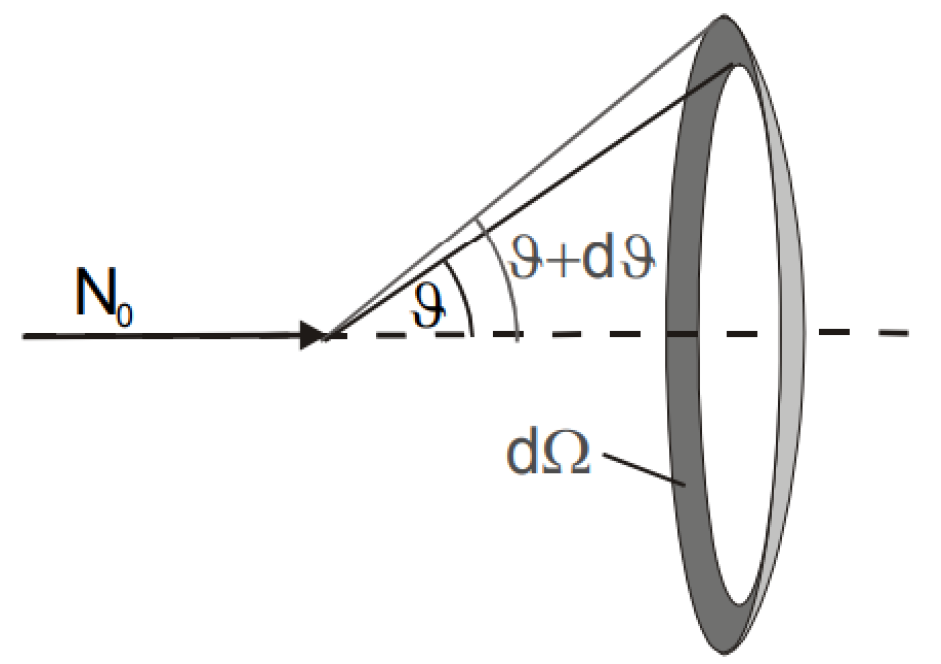
\includegraphics[width=0.6\columnwidth]{images/angle.png}
    \caption{Angular deflection of $\alpha$-particles, scattered into an angular region $\theta + d\theta$ and $\phi$ from 0 to $2\pi$}
    \label{2}
\end{figure}

The plane angular differential $d\theta$ corresponds
in three dimentions to a $d \Omega = 2\pi\sin\theta d\theta$.
Hence the space correction to $N_d(\theta)$ and the spatial
scattering rate $N(\theta)$ is

\begin{align} \label{eq:4}
    N(\theta) = \frac{N_d(\theta)}{2\pi\sin\theta}
\end{align}

\subsection{Determination of Unknown Nuclear Charge}

By keeping all quantities unchanged and by swapping the goild foil with a foil of an unknown material, we can find the atomic number of this unknown material. In this experiment for example, we have used Aluminium as the unknown element. From Eq. \ref{eq:2}, we can see that 

\begin{align*}
    N(\theta) \propto dZ^2
\end{align*}

where $d$ is the thickness of the foil and $Z$ is its atomic number. Hence for two materials of different thickness and atomic number (say Au and Al),

\begin{align} \label{eq:part2}
    \frac{Z_\text{Al}}{N_\text{Au}} &= \frac{d_\text{Al}Z^2_\text{Al}}{d_\text{Au}Z^2_\text{Au}} \nonumber\\
    \implies N_\text{Al} &= Z_\text{Au}\sqrt{\frac{d_\text{Au}N_\text{Al}}{d_\text{Al}N_\text{Au}}}
\end{align}

% =================================================
\section{Experimental Setup}

\subsection*{Apparatus}

\begin{enumerate}
    \item Rutherford Scattering chamber
    \item Au and Al foil with frames
    \item Vacuum pump
    \item Centering ring
    \item Discriminator preamplifier
    \item Counter
    \item Plug-in power supply unit 12 V
    \item Measuring cable BNC\\
\end{enumerate}

The experimental set-up consists of a scattering chamber
which holds the gold leaf and the detector, a discriminator
preamplifier, and a counter (Fig. \ref{3}). There is a vacuum pump attached to the scattering chamber as there might be a small number of alpha-particles in the air. The gold foil receives the alpha particles that are released from the Am-241 preparation through a slit
aperture, which exit the gold foil at varied scattering angles. A semiconductor detector is used to determine which alpha particles were
dispersed. With the arrangement we’re using, the gold
foil, slit, and preparation -- which are all mounted to a
standard swivel arm -- are what are swung, not the detector. The chamber’s side wall is securely fastened to the
detector. The discriminator level should be set halfway
between the spots where the noise is masking out and
where the alpha count rate starts to decline.

The discriminator preamplifier is set to a voltage such that the count rate is zero in around 100s for an angle $\sim$ 30, to eliminate any electrical noise.

\begin{figure}
    \centering
    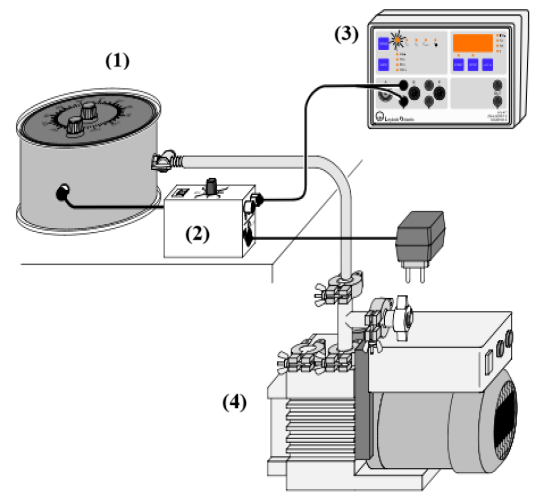
\includegraphics[width=1\columnwidth]{images/expt.png}
    \caption{The experimental setup with the (1) scattering chamber (2) discriminator preamplifier (3) counter and (4) vacuum pump}
    \label{3}
\end{figure}